\documentclass[a4paper, 11pt]{article}

\usepackage[utf8]{inputenc}
\usepackage{graphicx}
\usepackage{amsmath}
\usepackage{amsfonts}
\usepackage{hyperref}
\usepackage{pgf,tikz}
\usepackage{wrapfig}

\title{M1 Project - Image}
\author{Simon Mauras}
\date{March 29,  2016}

\begin{document}

\maketitle

\tableofcontents

\newpage
\section{Introduction}

\section{Implementation}

\subsection{Installation}
To install our shape classifier, you will need to install several Python 3 packages (scipy, numpy, sklearn). You will also need the C++ library \href{http://dgtal.org}{DGtal}.

\medskip\noindent To compile our project you need to have cmake installed.
\begin{verbatim}
mkdir build && cd build
cmake .. -DDGtal_DIR=/path-to-dgtal-folder/build
\end{verbatim}

\subsection{Feature extraction}

The feature extraction is done in C++ using the library DGtal. The file \verb|features.cpp| provides several functions to extract a vector of features from an image. 
The program \verb|shape_indexing| takes as input an image and write a vector of values in $\mathbb R^d$ on the standard output.
The program \verb|shape_distance| computes the similarity between the vectors of features of two images and write it on the standard outut.
The python script \verb|classifier_corpus.py| builds a vector of feature for each image of the directory \verb|database| and store it in \verb|corpus.csv|.

\subsection{Machine learning}

Once we have extracted a vector of values for each image of the database, we train a learning model on the corpus. The script \verb|classifier_learning.py| reads the vectors of features, train a learning model and export it in the file \verb|model.dump|.

\noindent We choose to use a $k$-nearest neighbors classifier (\href{http://scikit-learn.org/stable/modules/generated/sklearn.neighbors.KNeighborsClassifier.html}{scikit-learn}).
To have an estimation of the score with the whole database, we use cross-validation.

\newpage
\section{Learning models}

As machine learning is not the objective of the project, this part will be brief. The goal of model selection is to find the best machine learning algorithm (and the best parameters) for our dataset. We tested several models ($k$-neighbors, Gaussian naïve bayes, Logistic regression, Decision tree, Random forest, \dots). To evaluate the score we use cross-validation. We chose to use a $k$-neighbors classifier with $k= 25$.


\subsection{$k$-nearest neighbors classifier}

Let's introduce the problem of machine learning. Given a set $E$ of points, each of them being labeled by a class $c \in C$. We assume that the distribution of the classes follows some pattern. We want an algorithm able to decide in which class a point $e \in E$ belongs. To do that, we are given a corpus $(X, y)$ with $X \in E^n$ a family of points and $y \in C^n$ the classes to which they belong. 

We chose the $k$-nearest neighbors classifier algorithm. For each query $e \in E$ we look for the $k$-nearest point to $e$ in $X$ (using a distance $d$). The class with the biggest frequency in this set of $k$ points is the most likely class. To compute efficiently the $k$-nearest neigbors of a point we typicaly store $X$ in a datastructure like a Kd-tree.

\subsection{Cross-validation}

Now that we have a learning algorithm, we want to evaluate its efficiency. But we only know the classes of the points of the corpus. And computing the score of our algorithm on the corpus is a very bad approximation. Indeed our algorithm may be very good inside the corpus and very bad outside of it. One solution to this problem is cross-validation ($N$-fold cross validation).
\begin{itemize}
	\item Shuffle the corpus, then split it in $N$ parts (of equal size).
	\item For each part, train the algorithm on the $N-1$ remaining parts and compute the score with the current one.
	\item Compute the average (or the minimum) of those scores.
\end{itemize}
We can expect that the score outside of the training corpus is close to the cross-validation score.


\newpage
\section{Normalization}

During the classification, we need to analyse some noisy images. A preprocessing is therefore needed. Our preprocessing is done in several steps.
\begin{itemize}
  \item Scale the image.
  \item Smooth with a median filter.
	\item Compute the contour of the shape.
	\item Fill-in the shape.
\end{itemize}

\noindent We normalize images using function \verb|normalize| (in \verb|features.cpp|).
The scaling is important because even if our features are scale-invariant, the digitization is a huge problem. Indeed after a few experiments, we realize that scaling then smoothing is better than just using the initial image. The result of normalization on a very noisy shape is satisfactory. 

\begin{figure}[h!]
\centering
\begin{tabular}{ll}
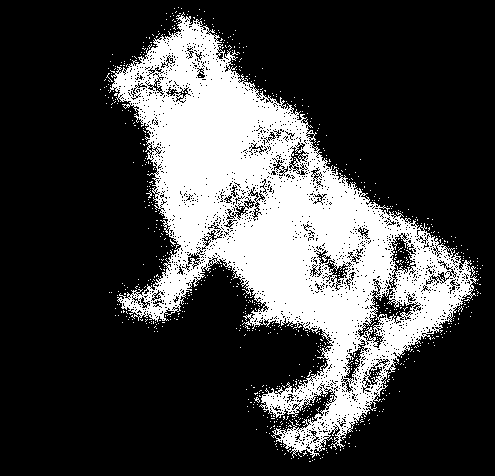
\includegraphics[width=4cm]{normalize-noisy-1.png} &
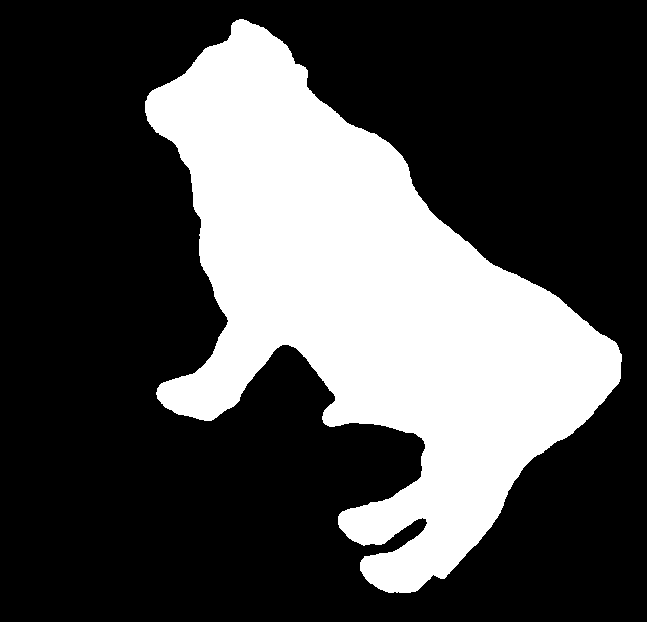
\includegraphics[width=4cm]{normalize-noisy-2.png} \\
\end{tabular}
\caption{Normalization of a noisy shape}
\end{figure}
 
\noindent If there are several connex components, the biggest one is choose to be the shape. The filling part of the normalization is very usefull for classes like butterfly, cattle or dog as some images contains a lot of gaps and other don't.

\begin{figure}[h!]
\centering
\begin{tabular}{ccc}
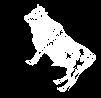
\includegraphics{normalize-1.png} &
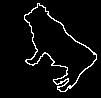
\includegraphics{normalize-2.png} &
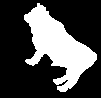
\includegraphics{normalize-3.png} \\
\end{tabular}
\caption{Filling the shape}
\end{figure}

\newpage
\section{Feature design}

\subsection{Distance Transformation Percentile}
Let's take a look at the distance transformation histogram for several shapes.
\begin{figure}[h!]
\centering
\begin{tabular}{ll}
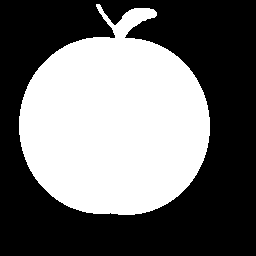
\includegraphics[width=5cm]{apple.png} &
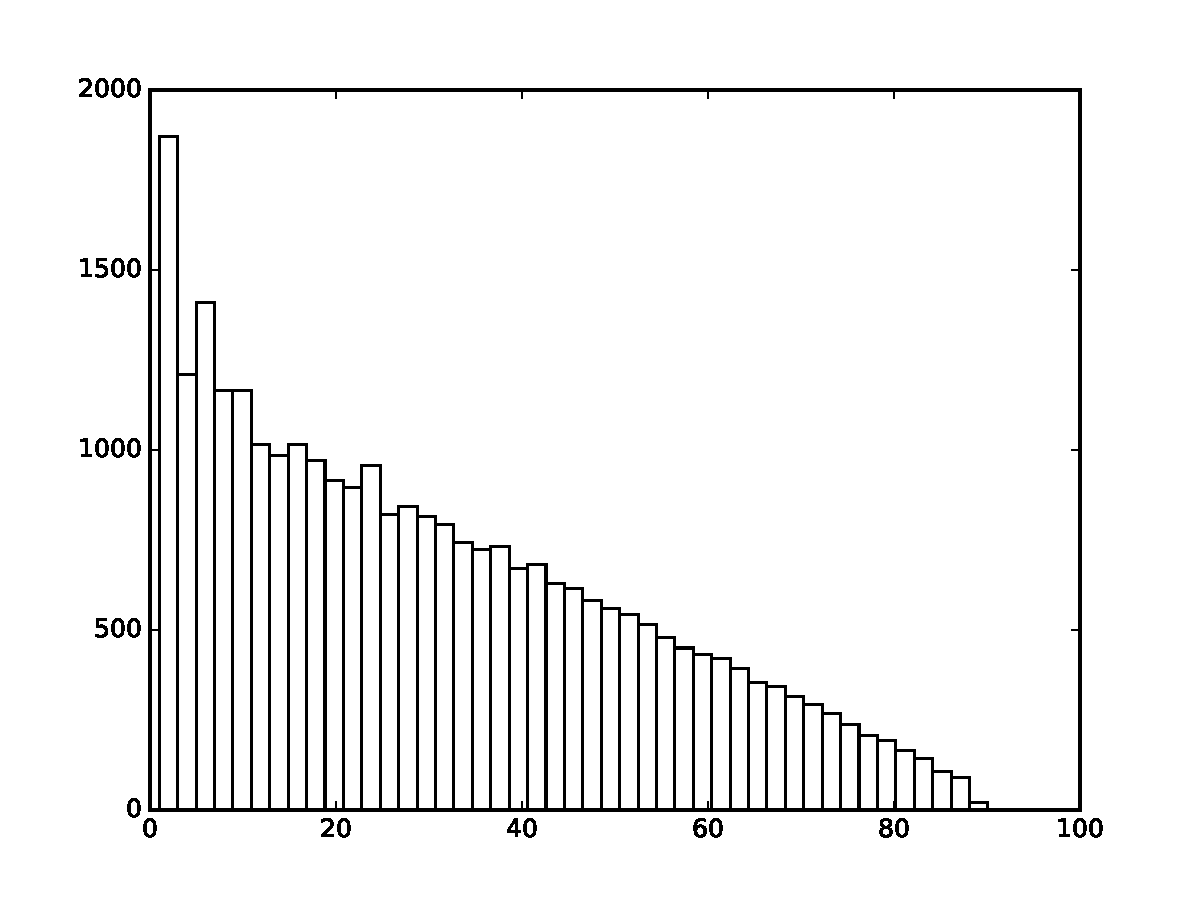
\includegraphics[height=5cm]{apple-dthist.pdf} \\
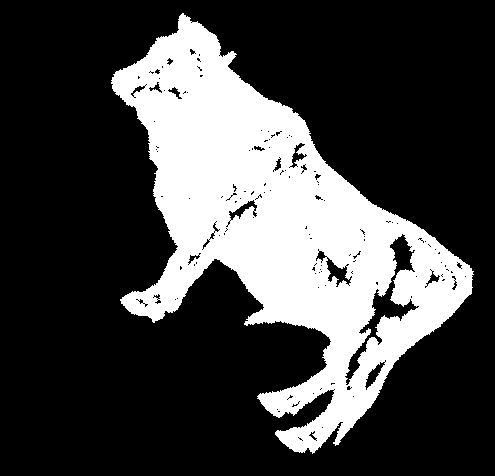
\includegraphics[width=5cm]{cattle.png} &
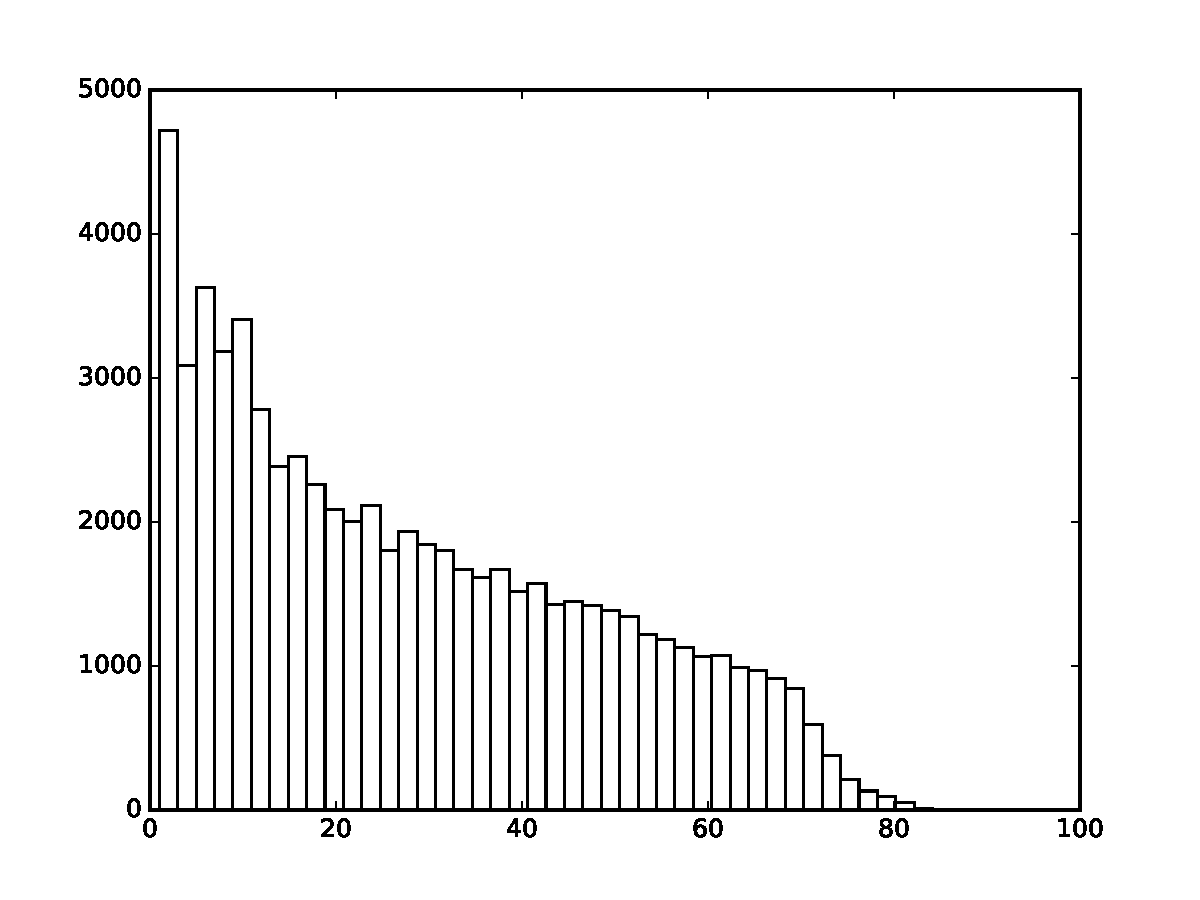
\includegraphics[height=5cm]{cattle-dthist.pdf} \\
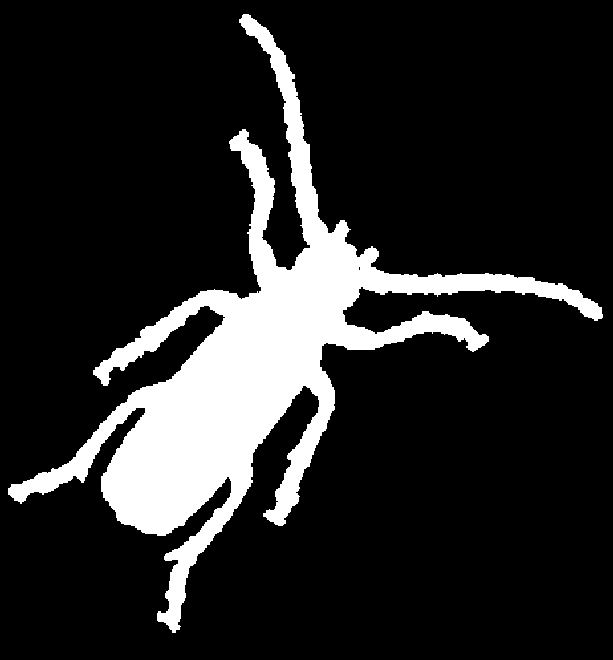
\includegraphics[width=5cm]{beetle.png} &
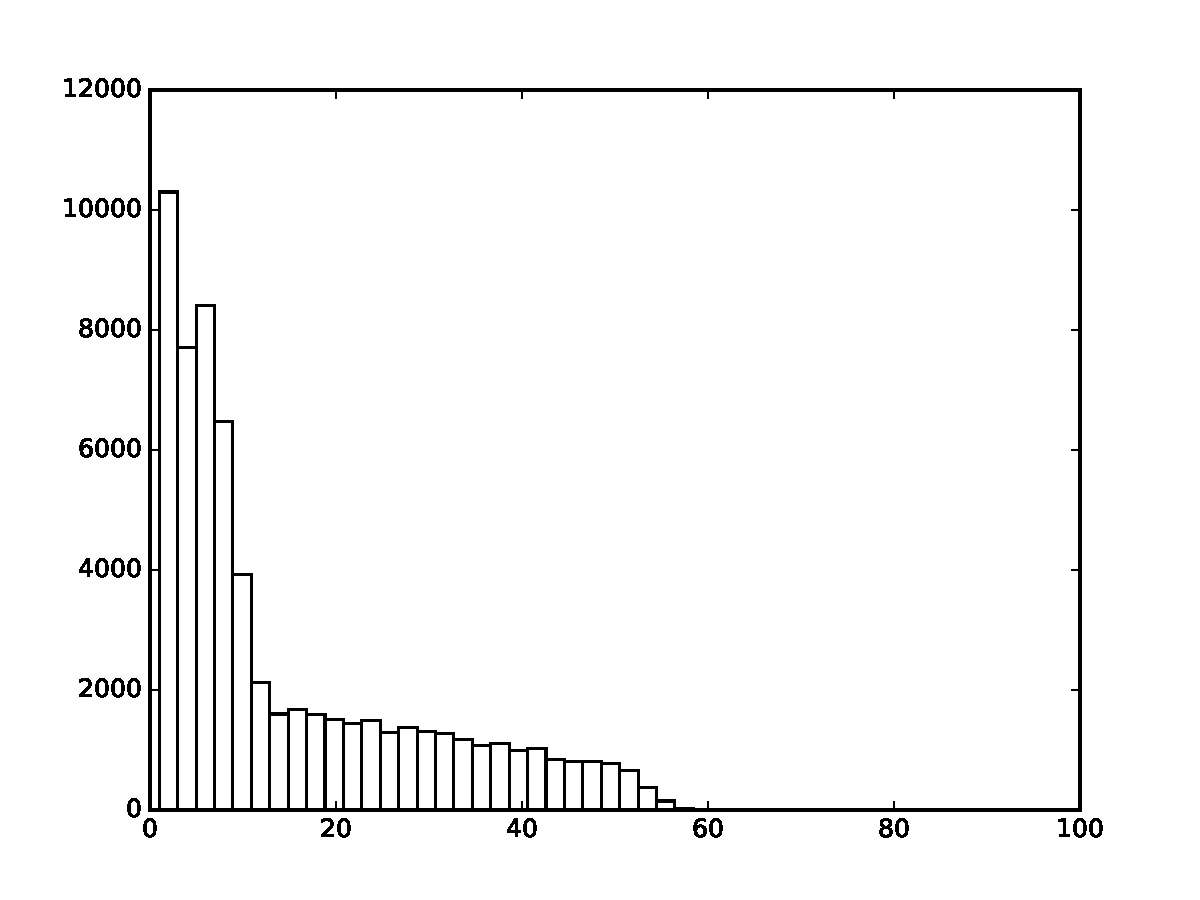
\includegraphics[height=5cm]{beetle-dthist.pdf} \\
\end{tabular}
\caption{Distance Transformation Histogram}
\end{figure}

\noindent We can observe that a shape can be characterized by the distributon of its distance transformation.

\noindent Now we need to build an estimator satisfying the following requirement:
\begin{itemize}
	\item Must be invariant under translation, scaling and rotation.
	\item We need some kind of continuity. If there is a small modification of the shape then the new estimation has to be close to the initial one.
\end{itemize}
We already have invariace by translation and rotation. In order to have the invariance under scaling, we can normalize the distance and the frequencies.

However we can notice that it is not enough to have a good estimator. Indeed the histograms $(1, 0, \dots, 0)$ and $(0, 1, 0, \dots, 0)$ are very close but the distance between those two vectors is huge. To fix this problem we are going to compute percentiles. The function \verb|compute_dt| (in \verb|features.cpp|) compute those features.
\begin{figure}[h!]
\centering
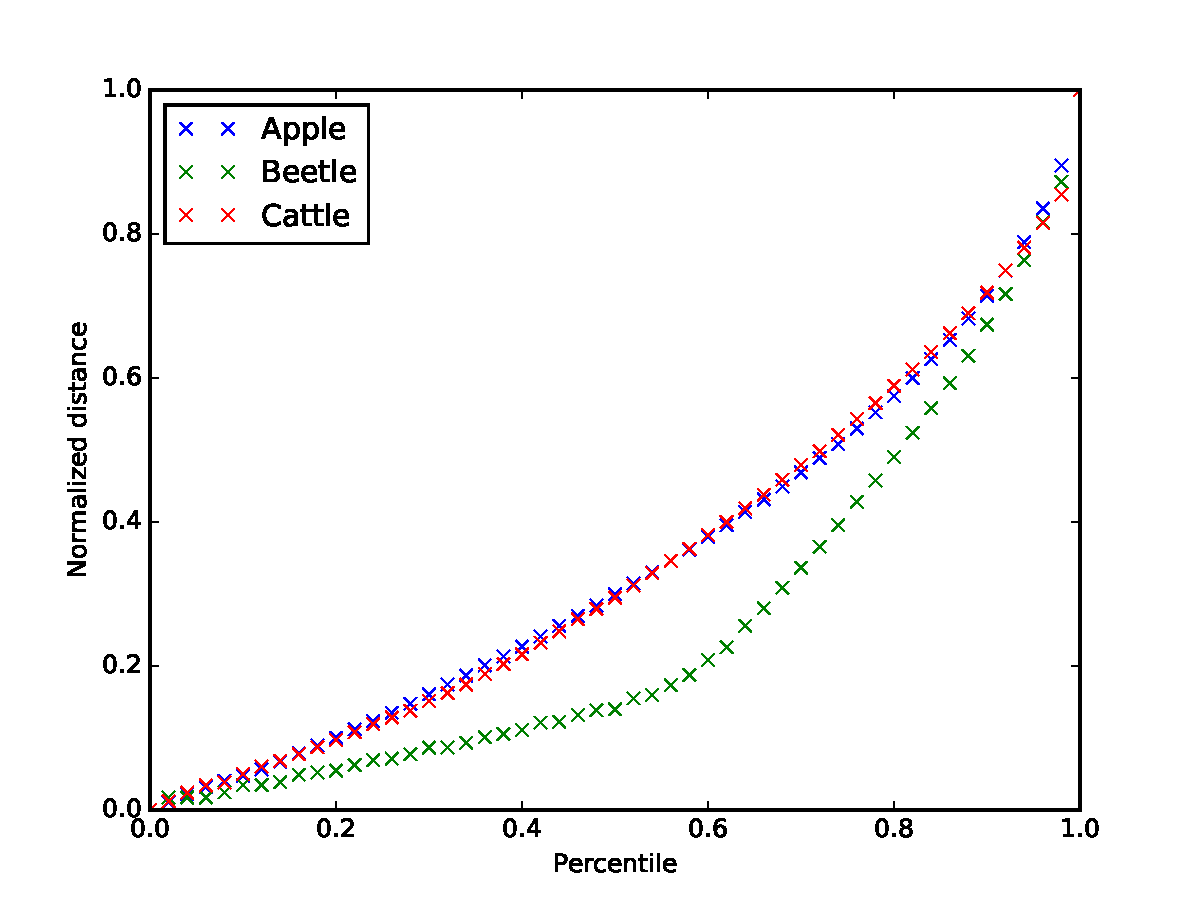
\includegraphics[width=13cm]{percentiles.pdf}
\caption{Distance Transformation Percentile}
\end{figure}

We just build an estimator that can help us to distinguish an apple from a beetle. But we can notice that this estimator is not very good to decide whether a shape is a cattle of an apple.

\newpage
\subsection{Perimeter and Area}
Among all the estimators we could implement, we chose to compute the perimeter and the area of the shape. However, a good feature must be invariant under scaling. When a shape is scaled by a factor $k$, all length are multiplied by $k$ and all areas are multiplied by $k^2$. So we add the perimeter over the square root of the area to the list of features.

\medskip It is implemented in the functions \verb|compute_area| and \verb|compute_perimeter| (in \verb|features.cpp|). We compute the perimeter by decomposing the contour into maximal DSS (DGtal implementation). We only compute the number of white pixels to evaluate the area of the shape.

\subsection{Rotation Distance}

One caracteristic which is still not used is point reflexion. There is a lot of images with symetry and rotation invariance. Our idea is to compare the initial image with its rotation of $\theta$ degrees around its centroid. We can prove that if we can find a invariance under rotation for our image, then the centroid of the shape will be the center of the rotation.

\medskip \noindent For $\theta = 2 \pi / k$ for $k = 2 \dots 10$ we chose to compute our features as follow:
\begin{itemize}
  \item Compute the centroid $c$ of the shape
	\item For each point $p$ of the shape
	\begin{itemize}
	\item Compute its rotation $q = c + e^{i\theta}(p - c)$
	\item If there is a point in the shape at distance to $q$ less than $r$,\\then add 1 to the score.
  \end{itemize}
  \item Normalize the score (divide by the number of pixels in the shape)
\end{itemize}

\noindent The function \verb|similarity_rotation| (in \verb|features.cpp|) implement the algorithm we just describe.

\medskip\noindent The figure \ref{figure:rotation} contains the value of those features for five different classes. When $k$ goes from 2 to 10, the angle goes from $\pi$ to $\pi / 10$.
We can recognize the $\pi/6$ rotation invariance of device 1 and the circular shape of an apple.
The results are very relevant for regular shapes (circles, squares, stars, ...). With distance transformation we had trouble to distiguish an apple from a cattle, now we can separate those two classes.

\begin{figure}[p]
\centering
\begin{tabular}{ll}
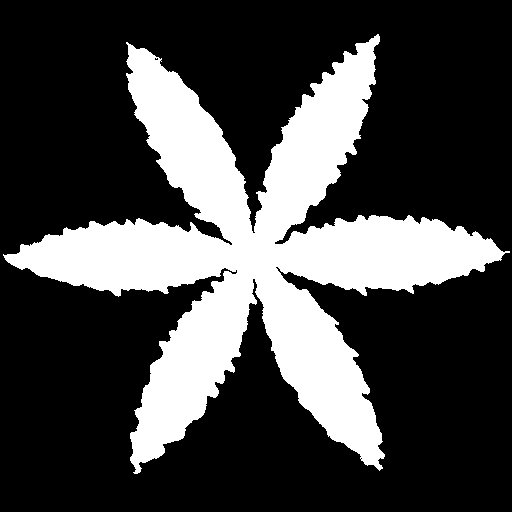
\includegraphics[width=4cm]{device1.png} &
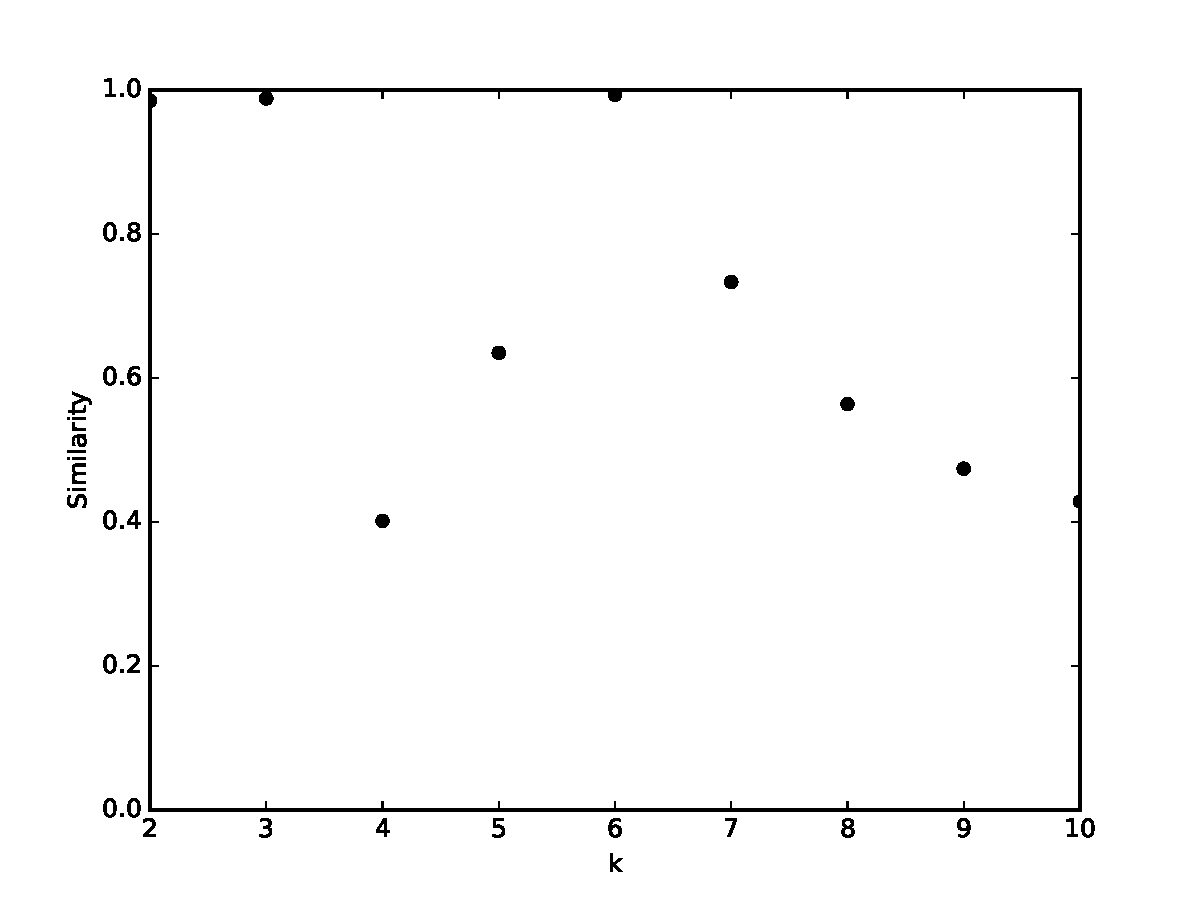
\includegraphics[height=4cm]{device1-rotation.pdf} \\
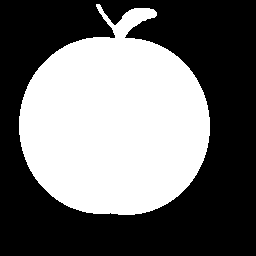
\includegraphics[width=4cm]{apple.png} &
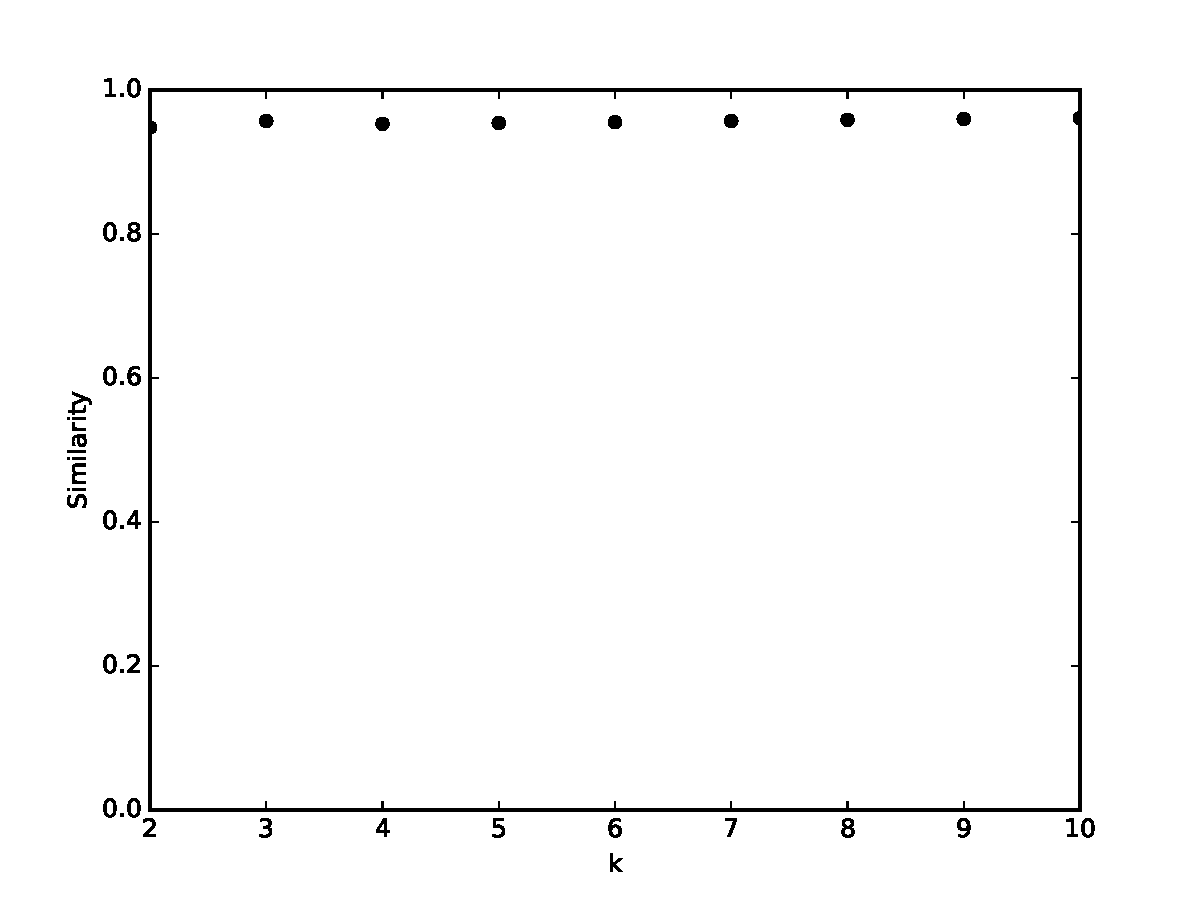
\includegraphics[height=4cm]{apple-rotation.pdf} \\
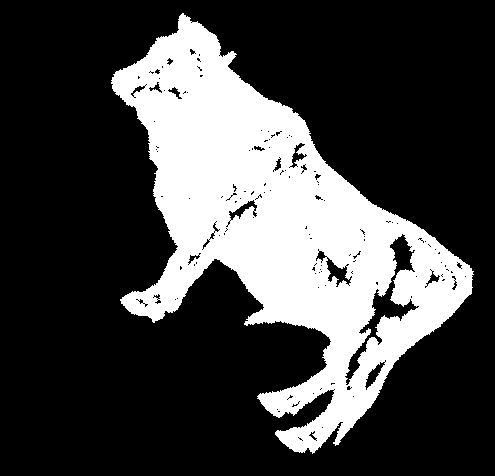
\includegraphics[width=4cm]{cattle.png} &
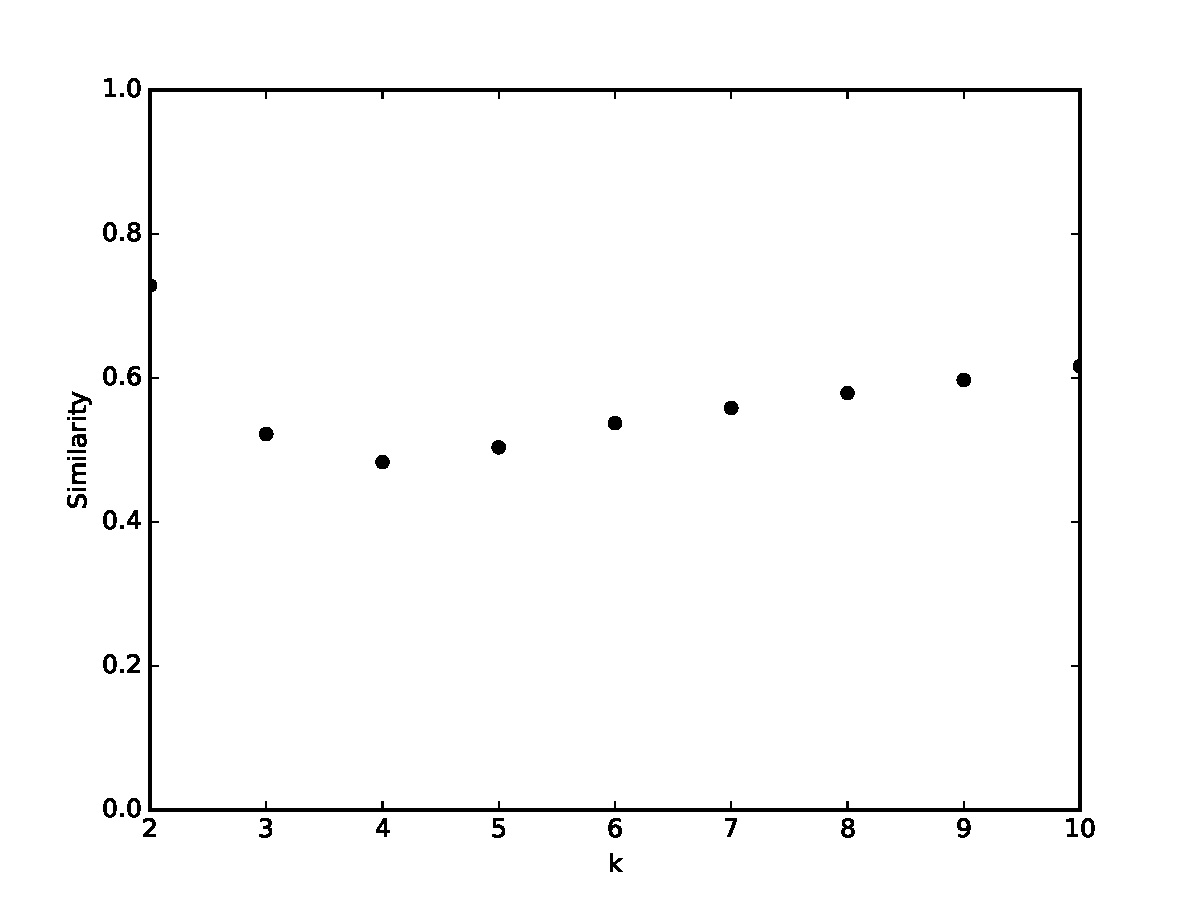
\includegraphics[height=4cm]{cattle-rotation.pdf} \\
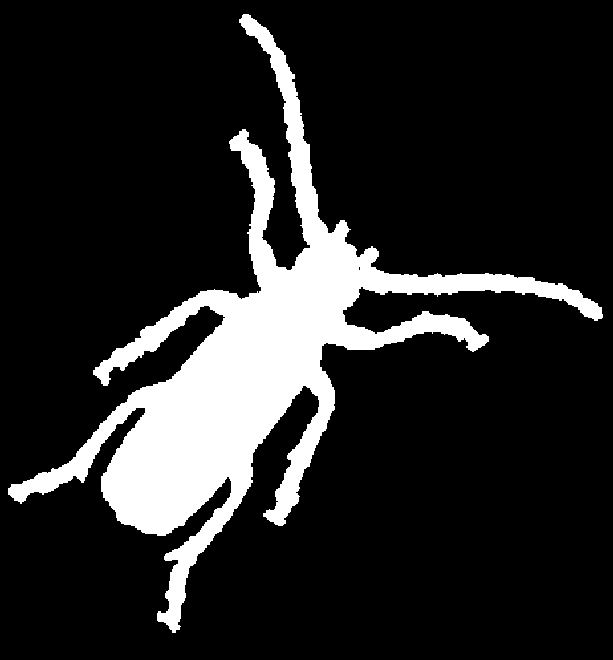
\includegraphics[width=4cm]{beetle.png} &
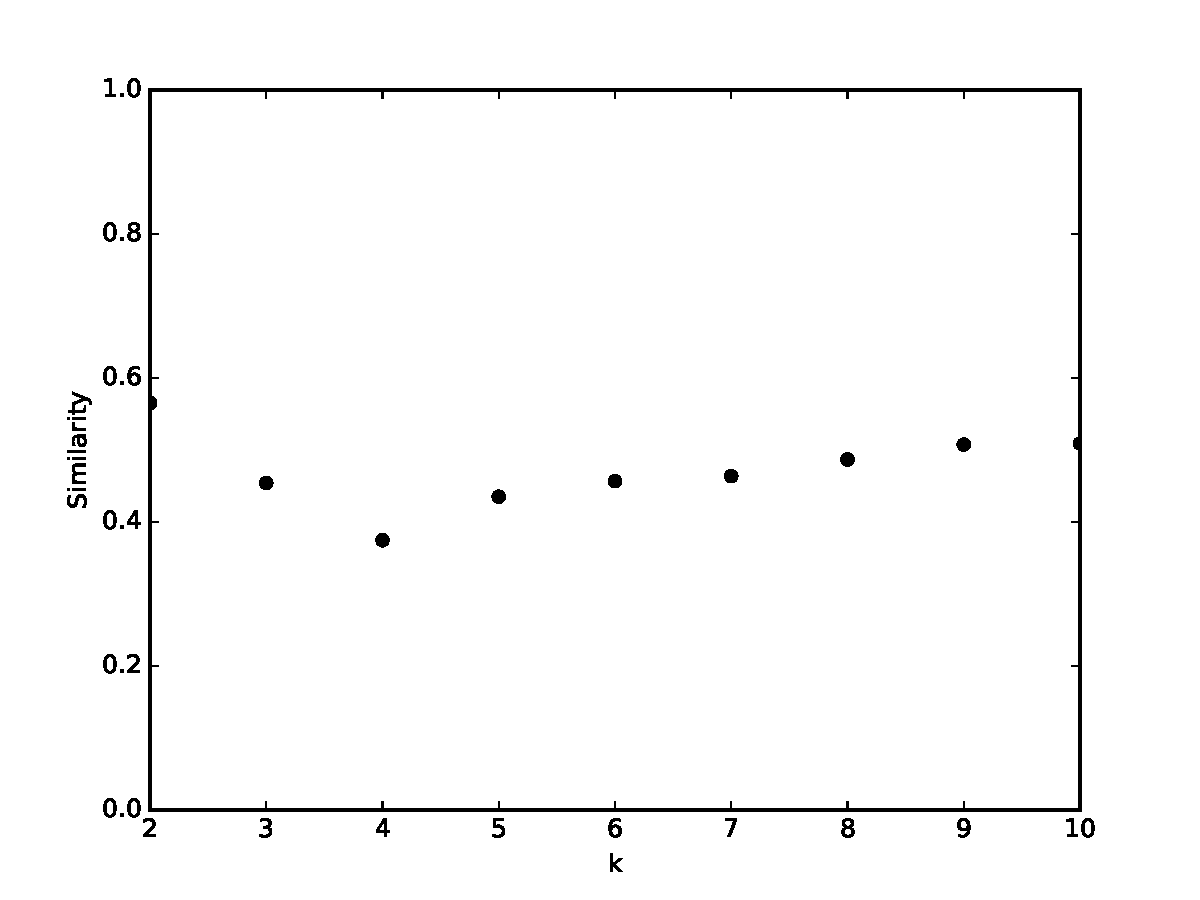
\includegraphics[height=4cm]{beetle-rotation.pdf} \\
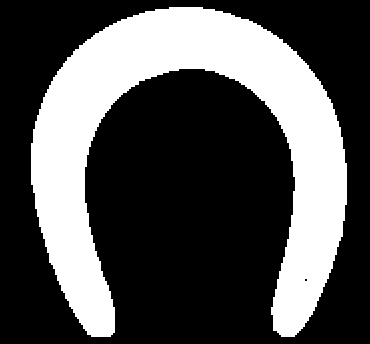
\includegraphics[width=4cm]{horseshoe.png} &
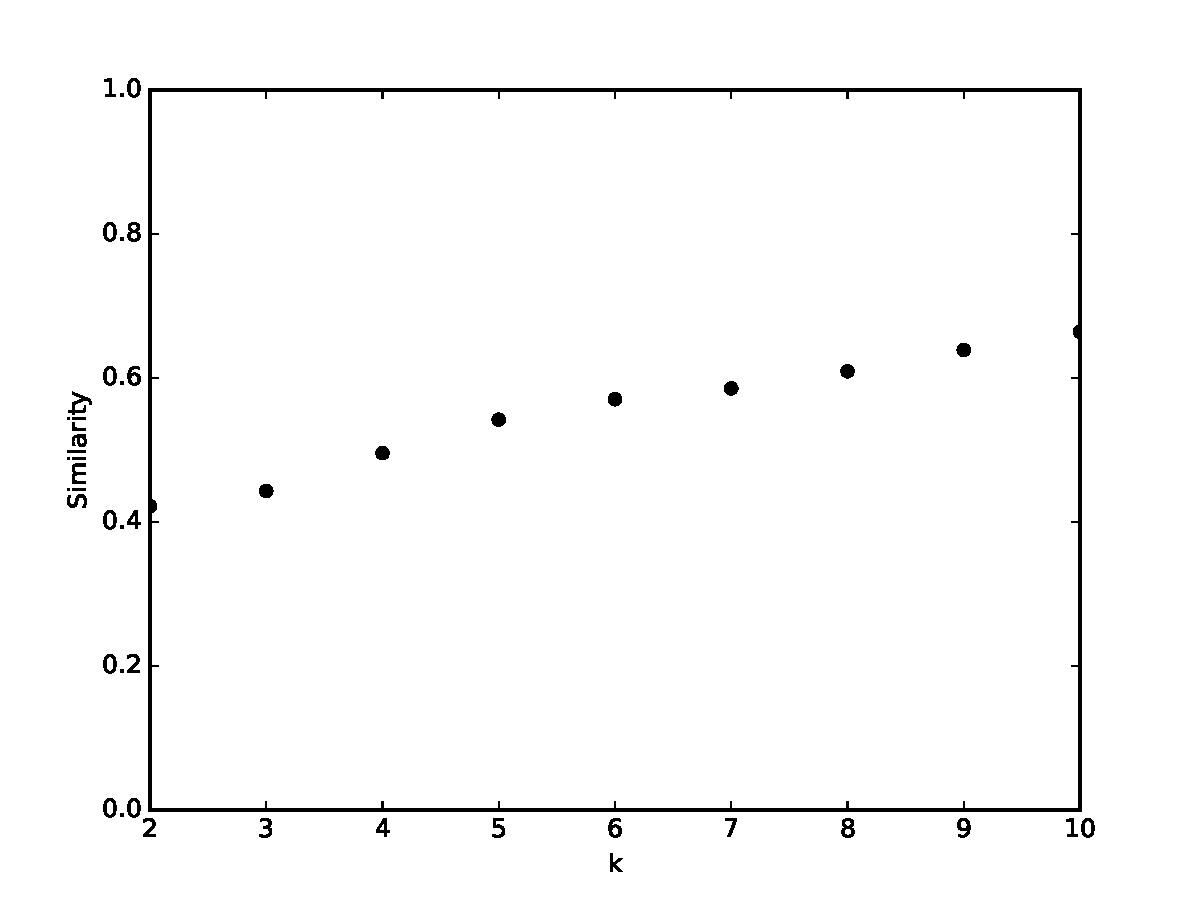
\includegraphics[height=4cm]{horseshoe-rotation.pdf} \\
\end{tabular}
\caption{Rotation Distance}
\label{figure:rotation}
\end{figure}

\newpage
\subsection{Convex hull}

The convex hull of a set of point $X$ is the smallest convex set that contains $X$. There exists several algorithms to compute the convex hull of a 2D finite set (Graham's scan, ...)
We implemented the function \verb|convex_hull| (in \verb|features.cpp|)  which computes the convex hull of a 2D shape in an image.

\begin{wrapfigure}{r}{6cm}
\centering
\definecolor{qqqqff}{rgb}{0,0,1}
\definecolor{ffqqqq}{rgb}{1,0,0}
\definecolor{cqcqcq}{rgb}{0.75,0.75,0.75}
\begin{tikzpicture}[line cap=round,line join=round,x=0.5cm,y=0.5cm]
\draw [line width=1.6pt,color=ffqqqq] (6,2)-- (7,4);
\draw [line width=1.6pt,color=ffqqqq] (7,4)-- (10,5);
\draw [line width=1.6pt,color=ffqqqq] (10,5)-- (14,4);
\draw [line width=1.6pt,color=ffqqqq] (14,4)-- (16,2);
\draw [line width=1.6pt,color=ffqqqq] (16,2)-- (17,0);
\draw [line width=1.2pt,color=qqqqff] (6,2)-- (7,0);
\draw [line width=1.2pt,color=qqqqff] (7,0)-- (9,-2);
\draw [line width=1.2pt,color=qqqqff] (9,-2)-- (12,-3);
\draw [line width=1.2pt,color=qqqqff] (12,-3)-- (14.92,-2.2);
\draw [line width=1.2pt,color=qqqqff] (14.92,-2.2)-- (17,0);
\begin{scriptsize}
\fill [color=black] (6,2) circle (1.5pt);
\fill [color=black] (8,3) circle (1.5pt);
\fill [color=black] (10,3) circle (1.5pt);
\fill [color=black] (7,0) circle (1.5pt);
\fill [color=black] (10,5) circle (1.5pt);
\fill [color=black] (13,3) circle (1.5pt);
\fill [color=black] (14,4) circle (1.5pt);
\fill [color=black] (12,2) circle (1.5pt);
\fill [color=black] (10,1) circle (1.5pt);
\fill [color=black] (12.86,-0.04) circle (1.5pt);
\fill [color=black] (9,-2) circle (1.5pt);
\fill [color=black] (12,-3) circle (1.5pt);
\fill [color=black] (11,-1) circle (1.5pt);
\fill [color=black] (14.92,-2.2) circle (1.5pt);
\fill [color=black] (17,0) circle (1.5pt);
\fill [color=black] (15,1) circle (1.5pt);
\fill [color=black] (16,2) circle (1.5pt);
\fill [color=black] (7,4) circle (1.5pt);
\fill [color=black] (12,4) circle (1.5pt);
\fill [color=black] (8,1) circle (1.5pt);
\fill [color=black] (9,-1) circle (1.5pt);
\fill [color=black] (13,-2) circle (1.5pt);
\end{scriptsize}
\end{tikzpicture}
\caption{Upper and lower hull}
\end{wrapfigure}

\medskip In the function \verb|convex_hull| (in \verb|features.cpp|) we implemented the monotone chain algorithm (aka Andrew's algorithm) as our points are aready sorted (2D matrix of $0/1$). We first compute the upper hull and the lower hull.
Then we simultaneously go through the domain, the upper hull and the lower hull to decide whether each point of the image is in the convex hull. The overall complexity is in $\mathcal O(n)$ where $n=a \times b$ is the size of the image.

\medskip One feature that give very good results is the ratio between the area of the initial image and the area of the convex hull of the shape. It is straighforward to show that this estimator is invariant under translation and rotation. We can also notice that the two area are multiplied by the same factor when scaling an image.

\begin{figure}[h!]
\centering
\begin{tabular}{c@{~}c}
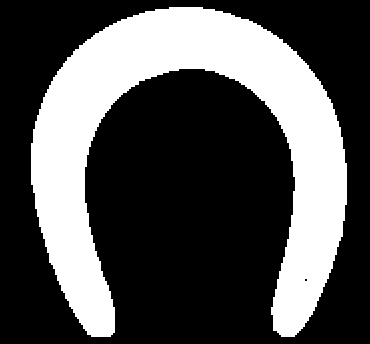
\includegraphics[height=3cm]{horseshoe.png} &
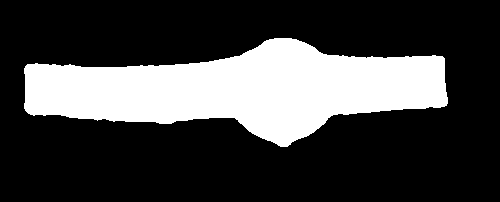
\includegraphics[height=3cm]{watch.png} \\
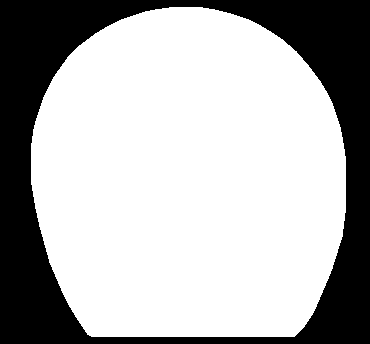
\includegraphics[height=3cm]{horseshoe-convex.png} &
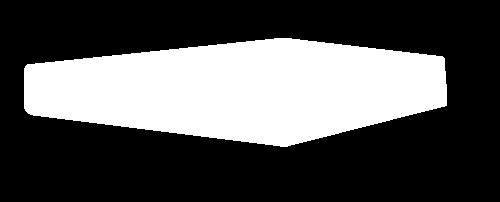
\includegraphics[height=3cm]{watch-convex.png} \\
Ratio = $0,46$ & Ratio = $0.79$
\end{tabular}
\caption{Convex Hull Area}
\end{figure}

 We also duplicated all the features we designed previously and used them on the convex hull of the shape.

\newpage
\section{Conclusion}

We have presented in this report the learning model we chose and the features we designed. Now is the time to analyse the results and the limits of our choices.

\subsection{Feature normalization}
The description of an image is a vector of values in $\mathbb R$. One first problem is that some of those values are bigger than others. More annoying, the variances are very different from one coordinate to one other. It is a problem as our learning model uses a "uniform" distance. We fix this problem manually by testing several weights for each feature.

\subsection{Robustness results}
The robustness of the feature extraction is an indicator showing how resistant to noise/scaling/rotation our features are. From one image we can construct an other one by rotating, scaling and adding noise. If we compute the feature vectors of those two images, their distance should be as small as possible. Let's define the similarity of two vectors $(u_i)_i$ and $(v_i)_i$.
\[\text{Similarity} = 1 - \max_i \frac{|u_i - v_i|}{|u_i| + |v_i|}\]
This definition is interesting because a good robustness certifies that for each coordinate the distance is small. (We use $\infty$ norm).
\begin{figure}[h!]
\centering
\begin{tabular}{|c|c|c|}
\hline
Noise & Robustness score & Variance \\
\hline
0.0 & 0.993 & $2.0 \times 10^{-4}$ \\
0.3 & 0.989 & $5.0 \times 10^{-4}$ \\
0.7 & 0.982 & $7.0 \times 10^{-4}$ \\
\hline
\end{tabular}
\caption{Robustness results}
\end{figure}

\subsection{Classification results}

We don't have the whole database of image so we can't know what our final score will be. However we have some hints. The cross validation score is supposed to be an approximation of the score of the classifier outsite of the training set. The cross validation score we get is $0.980$. As the robustness is close to $1$, we can expect a final score around $97\%$.

\end{document}